\section{Biological Background}

\begin{figure}[h]
  \centering
	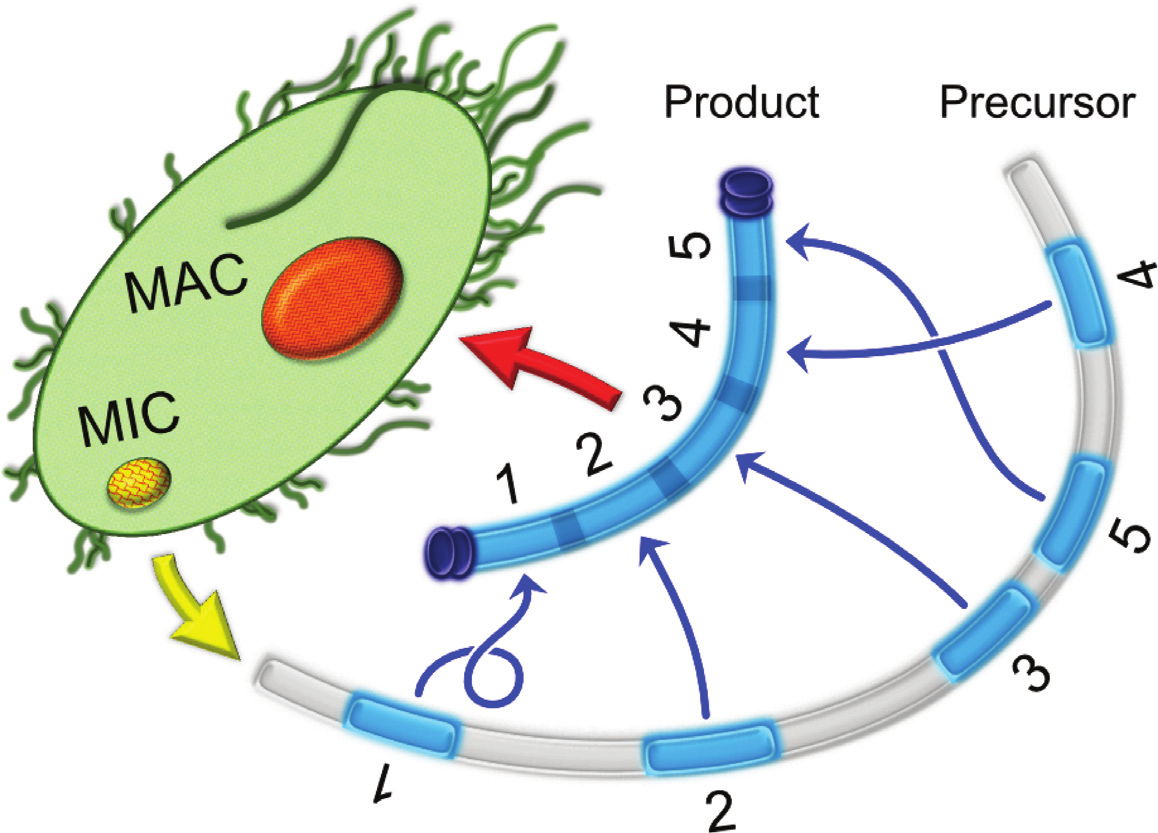
\includegraphics[width=250px]{0}
  \caption{In the somatic macronucleus (MAC), chromosomes assemble from precursor MDS building blocks (blue), which may be scrambled in some species. In the germline micronucleus (MIC), the Macronuclear Destined Sequences (MDSs) for all somatic chromosomes are dispersed over the long chromosome, and interrupted by Internally-Eliminated Sequences (IESs) and other noncoding DNA (gray). In some cases, an MDS may appear in a permuted order, or inverted\cite{mdsiesdb}.
}
\end{figure}

Ciliated protists (microbial eukaryotes using cilia for locomotion) exhibit nuclear dimorphism through the presence of separate germline and somatic nuclei. The somatic macronucleus (MAC) provides templates for the transcription of all genes required for asexual growth while the germline micronucleus (MIC) is used for the exchange of meiotic products during sexual reproduction \cite{mdsiesdb}. The MAC DNA is the one actively expressed and effectively results in the phenotype of the organism.

Several species of ciliates, such as \textit{Stylonychia} or \textit{Oxytricha}, go through extensive gene rearrangement while differentiating somatic macronuclei from germline micronuclei. This process entails an extensive fragmentation, elimination and sometimes broader rearrangement of the germline DNA, coupled to DNA amplification and telomere addition \cite{ciliatedDNA} and form the somatic macronuclei, all under the epigenetic control of novel non-coding RNA pathways \cite{programmedgenome}. The extent and the nature of these operations varies among ciliate species.

Each gene in the macronucleus may be present in the micronucleus as several nonconsecutive segments (macronuclear destined sequences, \textbf{MDSs}) separated by non-coding DNA. During macronuclear differentiation, the non-coding fragments (internal eliminated sequences, \textbf{IESs}) that interrupt MDSs in the micronucleus are deleted. Moreover, the order of the MDSs in the micronucleus may not be consecutive, in which case formation of the macronucleus requires unscrambling of the MDS order, as well as IES removal. There exist \textbf{pointer}-like sequences that are repeated at the end of the \textit{n}th MDS and at the beginning of the \textit{(n + 1)}st MDS in the micronucleus. Each pointer sequence is retained as only one copy in the sequence in the macronucleus \cite{ANGELESKA2007706}.

The general RNA-guided mechanism that regulate and lead this process of assembly is not known, theoretical investigations can be found in \cite{Brijder2007} and \cite{Ehrenfeucht:2004:CLC:971120}.


\section{Biological Motivation}
The guided genome rearrangement problem has (and it's) been extensively \cite{Ehrenfeucht:2004:CLC:971120} studied, both as biochemical process and mathematical model, as it provides an exaggerated case of a phenomenon observed among different species in different ways \cite{ANGELESKA20093020}. Similar broad scale, somatic rearrangement events occur in many eukaryotic cells and tumors.

Many discrete and topological models, mathematical approaches, biological and biochemical explanations and speculations on the theme can be found in literature (such as \cite{prescott2001} \cite{Brijder2014} \cite{ANGELESKA2007706} and \cite{programmedgenome}).

\section{Formalisation}

\begin{figure}[h]
  \centering
    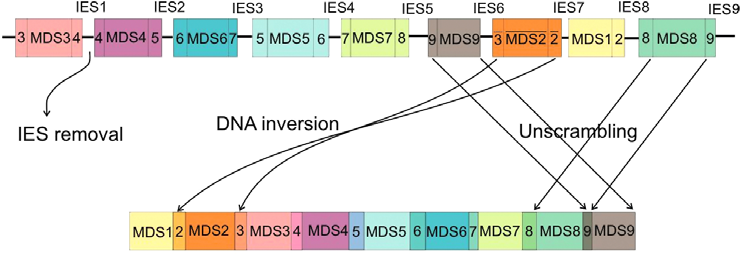
\includegraphics[width=\textwidth]{1}
  \caption{Schematic representation of the scrambled Actin I micronuclear germline gene in Oxytricha nova (top) and the correctly assembled macronuclear gene (bottom). Each block represents an MDS, and each line between blocks is an IES. The numbers at the beginning and at the end of each segment represent the pointer sequences. Note that MDS3-MDS8 require permutation and inversion to assemble into the orthodox, linear order MDS1-MDS9 in the macronucleus. The bars above MDS2 and its pointers indicate that this block is inverted relative to the others, i.e., this sequence is the Watson - Crick reverse complement of the version in the macronucleus; from\cite{prescottgreslin}.}

\end{figure}

The recognised events in the rearrangement process are:

\begin{itemize}
	\item The MAC begins a copy of the MIC DNA. The chromosomes are fragmented and amplified. The result of this process is the \textit{precursor}. $\sim$90\% of the complexity is lost.
	\begin{itemize}
    	\item Fragmentation
    	\item Amplification
    \end{itemize}

	\item From the precursor the final MAC DNA is produced through these further operations:
	\begin{itemize}
    	\item Elimination
    	\item Inversion
    	\item Gene Scrambling - Unscrambling
    	\item Telomere Addition
    \end{itemize}

\end{itemize}

We focus on the second phase, trying to map the following "building blocks":

\begin{itemize}
	\item \textbf{MDSs}, the contiguous sequences copied, inverted or (order) scrambled in the MAC;
	\item \textbf{IESs}, sections not present in the MAC;
	\item \textbf{Pointers}, overlap sections between MDSs in the MAC (maybe inverted), present in multiple copies in the MIC;
\end{itemize}

The "inverse", "reverse", "reverse complement" terms refer to the \textit{Watson-Crick reverse complement} of the sequence.

The goal is to produce a \textit{rearrangement map}: a set of disjoint substrings representing the building blocks, eventual operations they will go through the process (scrambling, inversion) and their "destination" on the produced genome.

\subsection{Real Instance}

Ideally, we want to reach an approach capable of treating the entire MAC and MIC sequenced genomes of \textit{Oxytricha trifallax} or \textit{Tetrahymena thermophila}, available publicy \href{http://oxytricha.princeton.edu/mds_ies_db/}{online} in the \textsc{mds\_ies\_db} ("A database of macronuclear and micronuclear genes in spirotrichous ciliates" \cite{mdsiesdb}).

\textit{Oxytricha trifallax} has a 487.14 000 000 M long MIC sequence, rearranging in a 71.47 M characters long MAC \cite{mdsiesdb}.

Formally, given an initial genome(MIC or MAC precursor) and a rearranged one (MAC) the program produces an annotation map of the process the input has been through.

\section{Existent Approaches}

\cite{mdsiesdb} proposes an annotation map, built using this algorithm:

\cite{ANGELESKA20093020} 

\section{Formulation}

\subsection{Reduced Artificial Instance}
Working on the entire genomes would be prohibitive for such approach, and many of the existent solutions make assumptions on the nature of the genomes, as we've seen.

We take into consideration a reduced instace, designing a Python script which procedually generates an instance of the problem with given specific characteristics.

\subsection{Preprocessing}
\subsection{ILP}
The entire software and documentation produced during the Stage experience and the thesis drafting, including initial and discarded attempts are available in a public Git \href{https://github.com/avivace/dna-recombination}{repository} \cite{avivace_repo} on GitHub.

\section{Tools}
The experimental work of the Stage experience was done on a GNU/Linux Debian \texttt{buster/sid} workstation, making large of use of the shell and other tools:

\texttt{Git}, a distributed version control system, helped to keep track of every progress in the documents and the software produced.

\texttt{Python} \cite{Rossum:1995:PRM:869369} and its \texttt{IDLE} was used to quickly implement and experiment the algorithms and procedures. It's also the interface to the Gurobi interactive shell. \texttt{Ruby} was considered too.

\texttt{Gurobi Optimizer} \cite{gurobi} is a commercial optimization solver. It provides a Python interface to formulate linear problems and solve them within Python scripts.

The \texttt{TeX} typesetting engine (in the \texttt{LaTex} macros environment, with some some extensions like \texttt{BiBTex} and the \texttt{pdflatex} compiler) were used to produce the documentation, the thesis and the slides.

\section{List of produced software}
The list of produced software follows. A copy is available at \cite{avivace_repo}.
\begin{itemize}
	\item \texttt{gen.py} - generate reduced artificial instances and produce rearrangement maps (\ref{gen}).
	\item \texttt{rmapSchema.json} - proposed rearrangement map JSON schema (\ref{rmap}).
	\item \texttt{rmap.py} - example functions to parse and apply the rearrangement map format described in \ref{rmap}.
	\item \texttt{segment.py} - dynamic programming algorithm to compute every substring of a sequence.
	\item \texttt{ilp.py} - tentative Gurobi implementation of the proposed ILP formulation.
\end{itemize}

\section{Reduced artificial instance}
\label{gen}

Working on the entire genomes sequences would be prohibitive for such approach, and many of the existent solutions make assumptions on the nature of the genomes, as we've seen.

We take into consideration a reduced instance, considering a shorter sequence and only the main events (Scrambling, Inversion, Overlapping, Deletion).

A Python script which \textit{procedurally} generates an instance of the problem with given specific characteristics has been developed, it takes the following parameters to shape the desired instance:

\begin{itemize}
	\item MIC length
	\item MDS quantity
	\item Overlap size
	\item Inverse rate
\end{itemize}

The generated instance consists in:

\begin{itemize}
	\item A (randomized) MIC DNA sequence
	\item A rearrangement map containing positions, inversion flags and annotation for every MDS, Pointer in both MIC and MAC
	\item The resulting MAC sequence
\end{itemize}

\clearpage

Running \texttt{\$ python gen.py}, we get:
\begin{verbatim}
Generated instance:

MDS     Start   End
0       3       9
1       21      27
2       30      38
3       40      50
4       13      19

P       Start1  End1    Start2  End2
1       7       9       21      23
2       25      27      30      32
3       35      38      40      43
4       46      50      13      17

MIC     ---AAATAT----TGGAGG--ATCGGT---GTAGAATT--ATTTCGTGGA----------
               ^^    ^^^^    ^^  ^^   ^^   ^^^  ^^^   ^^^^
MAC     AAATATCGGTAGAATTTCGTGGAGG
            ^^  ^^   ^^^   ^^^^
\end{verbatim}
The parameters used were:

\begin{itemize}
	\item $60$ as MAC length
	\item A random value in the $2-5$ range as MDS quantity
	\item $0$ as Inverse rate
	\item $30\%$ as Overlap size
\end{itemize}

The pointer regions are marked in both MIC and MAC. IESs are masked for clarity. The complete annotation map is exposed through four produced objects: \texttt{MDS\_MAC}, \texttt{MDS\_Mic}, \texttt{Pointer\_MIC} and \texttt{Pointer\_MAC}, easily navigable to fetch any information about the simulated process, e.g., \texttt{Pointer\_MIC[1]["Start2"]} and \texttt{Pointer\_MIC[1]["End2"]} gives the position of the second occurrence of the first pointer section in the MIC. A standard JSON object, serializing this data, is produced, too.

\subsection{(Proposed) Rearrangement map format}
\label{rmap}
Here we show a simple rearrangement map format adopted in this work. A specification gives a coherent and reliable way interpret the events represented by the map.
A JSON schema of the format specification is proposed in \texttt{rmapSchema.json} and it's further documented on the example library that handles it (\texttt{rmap.py}).

The necessity to \textit{apply} them on genomes and produce simulations is described in \ref{correctness}.

The following events can be described:

\begin{itemize}
	\item Deletion. Implicit and trivially computable.
	\item Scrambling. The array index represents the final ordering in the MAC. Implicit, the scrambled order can be computed using the \texttt{start} and \texttt{end} positions.
	\item Overlapping of pointer sections. A pointer section is a sequence common to 2 MDSs. The pointer can appear inversed in one or both occurrences.
	\item Inversion. An MDS can appear in the resulting genome as the Watson-Creek reverse complement version of the one in the MIC.
\end{itemize}

Here's how a rearrangement map in this format looks like, generated by \textit{gen.py}.

\begin{verbatim}
{
  "mac_length": 18,
  "mic_length": 60,
  "mds": [
    {
      "start": 27,
      "end": 32,
      "inverted": 0
    },
    {
      "start": 3,
      "end": 10,
      "inverted": 0
    },
    {
      "start": 14,
      "end": 24,
      "inverted": 0
    }
  ],
  "pointers": [
    {
      "start1": 30,
      "end1": 32,
      "start2": 3,
      "end2": 5
    },
    {
      "start1": 8,
      "end1": 10,
      "start2": 14,
      "end2": 16
    }
  ]
}
\end{verbatim}

This file can now be used by \texttt{rmap.py} which reproduces the events described by the map on a given genome.
\clearpage
\section{ILP formulation}
A tentative \textit{pure} integer linear programming formulation follows.

\subsection{Variables definitions}

$*Eq(i,j,h,l) = \begin{cases} 0 \\ 1, & \mbox{if } \code{MIC[i:j]} = \code{MAC[h:l]} \end{cases}$ \\\\\\
$*cwc(i,j,h,l) = \begin{cases} 0 \\ 1, & \mbox{if \code{MIC[i:j]} is the reverse complement of \code{MAC[h:l]}} \end{cases}$ \\\\\\
$MDS_{MICstart}(i,j) = \begin{cases} 0 \\ 1, & \mbox{if MDS } i\mbox{ starts at position } j \mbox{ in the MIC} \end{cases}$ \\\\\\
$MDS_{MICend}(i,j) = \begin{cases} 0 \\ 1, & \mbox{if MDS } i\mbox{ ends at position } j \mbox{ in the MIC} \end{cases}$ \\\\\\
$MDS_{MACstart}(i,j) = \begin{cases} 0 \\ 1, & \mbox{if MDS } i\mbox{ starts at position } j \mbox{ in the MAC} \end{cases}$ \\\\\\
$MDS_{MACend}(i,j) = \begin{cases} 0 \\ 1, & \mbox{if MDS } i\mbox{ ends at position } j \mbox{ in the MAC} \end{cases}$ \\\\\\
$Inv(i) = \begin{cases} 0 \\ 1, & \mbox{if MDS } i\mbox{ is inverted in the MAC } \end{cases}$ \\\\\\
$P_{start}(i,j) = \begin{cases} 0 \\ 1, & \mbox{if } MDS_{MACstart}(i,j) = 1 \mbox{, Pointer } i \mbox{ starts at position } j \mbox{ in the MAC} \end{cases}$ \\\\\\
$P_{end}(i,j) = \begin{cases} 0 \\ 1, & \mbox{if } MDS_{MACend}(i-1,j) = 1 \mbox{, Pointer } i \mbox{ ends at position } j \mbox{ in the MAC} \end{cases}$ \\\\\\
$Cov_{MACPOINT}(i,j) = \begin{cases} 0 \\ 1, & \mbox{if Pointer i covers the position j in the MAC} \end{cases}$ \\\\\\
$Cov_{MIC}(i,j) = \begin{cases} 0 \\ 1, & \mbox{if MDS } i\mbox{ covers the position } j \mbox{ in the MIC} \end{cases}$ \\\\\\
$Cov_{MAC}(i,j) = \begin{cases} 0 \\ 1, & \mbox{if MDS } i\mbox{ covers the position } j \mbox{ in the MAC} \end{cases}$ \\\\\\
Variables marked with $*$ will be populated during the preprocessing phase. \\\\\\

$\mbox{Objective Function:} \qquad min \mathlarger{\sum_{i,j} MDS_{MACstart}(i,j)}$

\subsection{Constraints}

\paragraph{MDS integrity and validity}MDSs must correspond to identical or reverse and complemented substrings of MIC and MAC. The following constraints enforce this fact:
\\\\\\
$(1) \qquad MDS_{MICstart}(i,a) + MDS_{MICend}(i,b) + MDS_{MACstart}(i,c) + MDS_{MACend}(i,d) + Inv(i) \leq 5 cwc(a,b,c,d) \label{eq:someequation} \qquad \forall i,a,b,c,d$ \\\\\\
$(2) \qquad MDS_{MICstart}(i,a) + MDS_{MICend}(i,b) + MDS_{MACstart}(i,c) + MDS_{MACend}(i,d) \leq 4 Eq(a,b,c,d) \qquad \forall i,a,b,c,d $ \\\\\\
$(3) \qquad \mathlarger{\sum_{j} MDS_{MICstart}(i,j)\leq 1 \qquad \forall i}$ \\\\\\
$(4) \qquad \mathlarger{\sum_{j} MDS_{MICend}(i,j) = \sum_{j} MDS_{MICstart}(i,j) \qquad \forall i}$ \\\\\\

\paragraph{Coverage} $ $
\\\\\\
$(5) \qquad \mathlarger{\sum_{l\leq j} MDS_{MICstart}(i,l) + \sum_{l\geq j}MDS_{MICend}(i,l) - 2Cov_{MIC}(i,j) = 0} \qquad \forall i,j $ \\\\\\
$(6) \qquad \mathlarger{\sum_{l\leq j} MDS_{MACstart}(i,l) + \sum_{l\geq j}MDS_{MACend}(i,l) - 2Cov_{MAC}(i,j) = 0} \qquad \forall i,j $ \\\\\\

\paragraph{Pointer Regions} $ $
\\\\\\
$(7) \qquad P_{start}(i,j) = MDS_{MACStart}(i,j) \qquad \forall i \neq 1$ \\\\\\
$(8) \qquad P_{end}(i,j) = MDS_{MACEnd}(i-1,j) \qquad \forall i \neq 1$ \\\\\\
$(9) \qquad Cov_{MACPOINT}(i,j) = \mathlarger{\sum_{b \geq j} P_{start}(i,b) + \sum_{e < j} P_{end}(i,e) \qquad \forall i}$ \\\\\\
$(10) \qquad \mathlarger{\sum_{i} Cov_{MAC}(i,j) \geq 1 \qquad \forall j }$ \\\\\\
$(11) \qquad \mathlarger{\sum_{i} Cov_{MAC}(i,j) \leq 2 \qquad \forall j }$ \\\\\\
$(12) \qquad \mathlarger{\sum_{i} Cov_{MAC}(i,j) - \sum_{i} Cov_{MACPOINT}(i,j) = 1 \qquad \forall j}$ \\\\\\

% FIXME: <=, > not <= =>.

\section{Preprocessing}
This part of the software computes the value for some of the variables, taking the instance as input.

Some of the defined variables are \textit{4-dimensional MIC length $\times$ MIC length $\times$ MAC length $\times$ MAC length} arrays. The necessity of a sparse data structure was immediately clear: \textit{Sparray}, a Python module \cite{sparray} for sparse n-dimensional arrays using \textit{dictionaries} supporting any number of dimensions and any size was chosen to support these variables.

The Read-Write performance on these objects is satisfying: 15 milion integer values are written in random indexes in a 150M $\times$ 150M $\times$ 150M $\times$ 150M \textit{4d sparray} in less than 20 seconds. The data can then be accessed using a notation similar to the standard array one (\texttt{Sparray[Index1, Index2, Index3, Index4]}). \textit{Eq} and \textit{cwc} are populated during this phase, with a naive iterative algorithm.

Here we encounter our first big limitation of a \textit{pure} linear programming approach. Populating \textit{Eq} and \textit{cwc} in our test instance (60 characters long MIC) was trivial but this task becomes so expensive it's infeasible with even genome sequences of more than 1000 characters.

The subsequences matching part must be approached with an high performing alignment tool like \textit{BLAST}.

\section{Gurobi Implementation}

Here is a simple Python example in order to illustrate the use of the Gurobi Python interface. The example builds a model, optimizes it, and outputs the optimal objective value. \\

\noindent Maximize $\qquad x + y + 2 z$ \\
Subject to $\quad x + 2 y + 3 z \leq  4$ $(c_0)$\quad and $x + y \geq 1 $ $(c_1)$\\
$\qquad x, y, z \qquad \text{binary}$ \\

\clearpage

On Python:

\begin{verbatim}
from gurobipy import *

try:
    m = Model("mip1")

    x = m.addVar(vtype=GRB.BINARY, name="x")
    y = m.addVar(vtype=GRB.BINARY, name="y")
    z = m.addVar(vtype=GRB.BINARY, name="z")

    m.setObjective(x + y + 2 * z, GRB.MAXIMIZE)

    m.addConstr(x + 2 * y + 3 * z <= 4, "c0")
    m.addConstr(x + y >= 1, "c1")

    m.optimize()

    for v in m.getVars():
        print(v.varName, v.x)

    print('Obj:', m.objVal)

except GurobiError:
    print('Error reported')
\end{verbatim}

Our model starts with variables definition:
\begin{verbatim}
[...]
MDS_Mic_Start = m.addVars(11, len(mic),
                              vtype=GRB.BINARY,
                              name="MDS_Mic_Start")
MDS_Mic_End = m.addVars(11, len(mic),
                            vtype=GRB.BINARY,
                            name="MDS_Mic_End")
Cov_Mac = m.addVars(11, len(mac), vtype=GRB.BINARY, name="Cov_Mac")
Cov_Mic = m.addVars(11, len(mic), vtype=GRB.BINARY, name="Cov_Mic")
[...]
\end{verbatim}

To define constraints we make large use of the \texttt{addConstrs} method:
\\
Add multiple constraints to a model using a Python generator expression. Returns a Gurobi \textit{tupledict} that contains the newly created constraints, indexed by the values generated by the generator expression \cite{gurobi}.
\clearpage
Here is how some constraints described in \ref{ilp_form} are translated in a Gurobi model: \\\\

\noindent $(3) \qquad \mathlarger{\sum_{j} MDS_{MICstart}(i,j)\leq 1 \qquad \forall i}$  \\\\\\
$(3b) \qquad \mathlarger{\sum_{j} MDS_{MACstart}(i,j)\leq 1 \qquad \forall i}$

\begin{verbatim}
m.addConstrs((sum(MDS_Mic_Start[i,a] for a in range(len(mic))) <= 1
                     for i in range(11)), name="3")

m.addConstrs((sum(MDS_Mac_Start[i,a] for a in range(len(mac))) <= 1
                     for i in range(11)), name="3b")
\end{verbatim}
\paragraph{}
\noindent $(10) \qquad \mathlarger{\sum_{i} Cov_{MAC}(i,j) \geq 1 \qquad \forall j }$ 
\begin{verbatim}
m.addConstrs((sum(Cov_Mac[i,j] for i in range(11)
                   for j in range(macl)) == macl), name="c10")
\end{verbatim}

The objective function: \\\\

\noindent $min \mathlarger{\sum_{i,j} MDS_{MACstart}(i,j)}$

\begin{verbatim}
m.setObjective((sum(MDS_Mic_Start[i,a] for a in range(0,len(mic))
                                       for i in range(0,11))),
                                       GRB.MAXIMIZE)
\end{verbatim}

11 is an upper limit of MDS quantity.

\clearpage
\section{Correctness}
\label{correctness}

\paragraph{Lemma.}
Suppose

$I$ to be an instance of the problem,

$P$ to be the ILP formulation associated to $I$,

$S$ to be an assignment to every variable of $P$ satisfying the constraints.

Then it's possible to build a solution for $I$ with cost equal to the objective function in $S$.

\paragraph{Proof.}
The idea is checking if \textit{S} produced by Gurobi is compatible with the known rearrangement map of the instance, i.e., if the solution proposed by Gurobi represents our DNA recombination events. "Applying" the computed map to the instance MIC should build an exact copy of the MAC.

The complete test workflow follows.

\begin{enumerate}
	\item Produce an \textit{artificial} instance \textit{I} of the problem with the software described in the \textit{Reduced artificial instance} section. By definition, this instance exhibits the rearrangement events we want to study (Scrambling, Overlapping, Deletion, Inversion) and it's a compliant instance of the formalised problem. A \textit{known} rearrangement map $R_1$ is produced too.
	\item Run the preprocess script on the generated instance and populate some of the variables of the ILP formulation associated to \textit{I}
	\item Run the Gurobi implementation of $P$ passing the populated variables. An assignment $S$ of every variable of the formulation will be computed.
	\item Build a rearrangement map $R_2$ using $S$.
	\item If $S$ is a solution then it $R_2$ maps the rearrangement events. It is possible to simulate those events on the instance MIC and exactly obtain the MAC. $R_2$ is comparable with $R_1$.
\end{enumerate}

Step 1 is described in \ref{gen} while steps 2-4 are handled in the \texttt{ilp.py} script. Step 5 is covered in \texttt{rmap.py} where we provide a function that computes a final rearranged sequence given an initial sequence and a (compliant) rearrangement map \ref{rmap}.

This entire procedure can be pipelined and automatized to allow running a variety of tests.
\clearpage


\section{Conclusions}
Among other problems, inequalities like $1$ and $2$ described in \ref{ilp_form} could not be used in Gurobi, being too memory aggressive. They had to be replaced with constraints built using native Gurobi methods, allowing more than bare linear algebra.

A \textit{pure} integer linear programming approach in this terms is clearly not successful, given the magnitude of the data to process and our choices.

A mixed approach should give better results: preprocessing the common substrings (BLAST) and producing possible instances consisting of compatible subsets of matching substrings speeds up the initial part and won't bloat the ILP formulation with huge matrices of data.

A scoring function must be designed to measure the quality of the possible maps: an ILP formulation could then optimize the problem.

Note that we (and other approaches like MIDAS \cite{midas}) use a greedy criteria for MDSs annotation: a solution with the largest possible MDSs annotation is considered the best, requiring a 100\% MAC coverage.

As far as we know the process could actually behave differently: new speculations and the availability of transitional genomes, showing the process during intermediate phases, could change this view.
\subsection{GUROBI Implementation}